\chapter{Main alternatives, Decision and Development of the best one}

\section{Orbits}
\import{sections/OrbitDesign/}{Ch2-OrbitalCoverage}
\import{sections/OrbitDesign/}{Ch3-ConstConfig}
\import{sections/OrbitDesign/}{Ch4-OrbitPerturbations}
\import{sections/OrbitDesign/}{Ch5-Decision}

\section{Space Segment Systems. Satellite Design}
\import{sections/SatelliteDept/}{SatDesign}

\section{Ground Segment Systems}
\import{sections/CommunicationsDept/}{Ch3-GroundSegmentDesign}

\section{Protocol Stack}
\import{sections/CommunicationsDept/}{Ch1-SpaceSegment}
\import{sections/CommunicationsDept/}{Ch2-GroundSegment}

\section{Launcher and Deployer}
\subsection{Launching System}
The aim of this section is the selection of a launching platform. First of all, a review of the available ones on the market is carried out, secondly a small group of launchers is chosen and finally, an optimization is developed in order to find the most suitable system. 

\subsubsection{Launch site and vehicle analysis}
A general research is done in order to filter all the launchers that can be discarded without any study. The result of this research is that there are seven potential rockets in the market capable of deploying the constellation as well as carrying out the replacement needs. The launchers can be divided in two categories: the powerful ones and the small ones. The first ones are capable of carrying heavy payloads, however they present high operation costs whereas the second ones are way more economic due to the reduced size. In addition, the small rockets are more focused on commercial flights without having to attend governmental issues. A table of this seven candidates is shown in the \cite[Chapter 1, Section 1]{annex2}.

Once this first selection is done, more accurate information is needed so as to reach a reliable conclusion. However, none of the enterprises shows its information on the Internet or any similar divulgation channel with the exception of Arianespace. Thus, all of them must be contacted to get the needed data. The same email is sent to all seven enterprises and several days later, three of them show interest in the Astrea constellation: Rocket Labs, PLDSpace and LEO Launch \& Logistics. Since the other enterprises do not answer the requests and, as a consequence, will not provide the necessary information, they can be directly discarded. Hence, the candidates list is reduced to those three who responded the enquire plus Vega, given that its information is available online. 

In order to find the most suitable option achieving the project objectives, it is thought to do an evaluation process following the Ordered Weighted Average (OWA) method . First of all, the required parameters for the decision have to be determined. According to the orbit design, the range of inclinations, the number of orbital planes and the range of heights must be taken into an account. Nevertheless, more parameters are needed in order to ensure a reliable result: cost per satellite, frequency of launchings per year and number of satellites deployed per launch. Both range of inclinations and number of satellites per launch act as a restriction due to the following two reasons. First, since orbital plane changes are very expensive and are out of consideration, the minimum number of launchings must equal the number of orbital planes. In addition, being capable of deploying the constellation with the minimum number of launchings is an adequate solution. This turns the number of CubeSats per launch into a restriction: the chosen launcher must be capable of launching at least the number of satellites in an orbital plane. Secondly, the inclination is considered a restriction by the fact that if a rocket is not capable of deploying a satellite in the desired inclination, it makes no sense to use it. 

Since the number of orbital planes is 8 and the inclination is 72$^{\circ}$, any launcher which doesn't fulfills one of this restrictions can be automatically rejected. 

Moreover, the following table contains all the information mentioned above which is helpful to compare the different launchers and see if they accomplish the basic features. 

\begin{table}[h]
\begin{center}
\begin{tabular}{|c|c|c|c|c|}
\hline
\bf{Parameters} & \bf{Rocket Lab} & \bf{PLD} & \bf{LEO L\&L} & \bf{Vega}\\
\hline 
\bf{Satellites/Launch} & 24 & 34 & 150 & 325 \\
\hline 
\bf{Inclination($^{\circ}$) } & {39.2 to 99} & {116 or 140} & {any} & {any}\\
\hline 
\bf{Cost/Satellite (US dollars)} & 240,000 & - & 266,667 & 100,000\\
\hline 
\bf{Orbital planes} & 1 & 1 & 1 & 1 \\
\hline 
\bf{Frequency/year} & 9 & 8 & 8 & 2 \\
\hline 
\bf{Range of heights (km)} & LEO & LEO & LEO & LEO\\
\hline
\end{tabular}
\end{center}
\caption{Criteria}
\end{table} 

It is important to point out that all the rockets available in the market can achieve the necessary amount of satellites per launch. Although all of them reach the height the CubeSats need, PLD does not attempt the inclination needed which is 72$^{\circ}$. As a result, this launcher is not appropriate for the project purpose and it is rejected. 

According to the remaining 3 candidates, all of them are adequate candidates, nevertheless there is a characteristic that may interfere with the mission goals. At first instance, the frequency per year has not been considered a critical parameter. Those have been chosen regarding orbital parameters only, however, although the frequency does not influence de capability of the rocket of deploying a CubeSat in the desired orbit, it can compromise the set up of the constellation and the posterior replacements. The lower the frequency is, the slower the deployment will be. Therefore, the frequency of the three remaining candidates must be analyzed. As seen in the table, Vega presents the lowest frequency (two launchings per year). This value is not acceptable due to the intention of deploying one single orbital plane per launch. The placement of the whole constellation would last four years, this mean that de first planes would be near their replacement time while the last ones would only have been nearly a year in orbit. Thus, Vega can also be discarded.
 
This leaves the selection with only two options: Rocket Lab and LEO Launch\&Logistics. An Ordered Weighted Average can be made between those two candidates taking the cost/satellite, the number of orbital planes, the frequency and the range of heights into account. Yet, they both present the same number of planes and range of heights, consequently the OWA can be done regarding only the two cost and frequency. The first has to be minimized and the second maximized. Since Rocket Lab presents best values in one parameter and the other (240,000 US dollars vs 266,667 and 9 launchings/year vs 8) there is no need to develop an OWA. In addition, an e-mail from Rocket Lab is received stating that a launch per week is achievable. Thus, the chosen rocket is Electron, from Rocket Lab enterprise. This rocket fulfills all the requirements of the constellation. 

As it is given in Rocket Lab payload users guide \cite{Guide2016}, Electron is a two stage light rocket constructed from carbon fiber composite. It is powered by ten Rutherford engines, all of them use liquid oxygen (LOX) and rocket kerosene. The first stage has nine out of the ten engines which generate 152 kN of thrust. The second one, has the remaining engine which produces 22 kN. The second stage contains the fairing where the payload is placed. Electron is 17 m long and its diameter is 1.2 m. It is capable of launching 24 3U CubeSats every week at a LEO orbit with a range of inclinations from 39.2 to 99 degrees. 

Rocket Lab facilities are located in New Zeland. The test laboratories are placed near the airport of Auckland and the launch site is in Mahia.

Finally, the cost per satellite is 240.000 US dollars or if the rocket is totally filled, 5.760.000 US dollars the entire launch. Some images of Electron are showed in the  \cite[Chapter 1, Section 1]{annex2}, a picture of the launching site is also showed.  %  Section 2: Launching System
\documentclass{article}
\usepackage{color}
\usepackage{graphicx}
\usepackage{multirow}
\usepackage{wrapfig}
\usepackage[export]{adjustbox}
\usepackage{caption}
\usepackage{subcaption}
\usepackage{gensymb}
\begin{document}
\section{Launching System}
The aim of this section is the selection of a launching platform. First of all, a review of the available ones on the market is carried out, secondly a small group of launchers is chosen and finally, an optimization is developed in order to find the most suitable system. 
	\subsection{Launch site and vehicle analysis}
A general research is done in order to filter all the launchers that can be discarded without any study. The result of this research is that there are seven potential rockets in the market capable of deploying the constellation as well as carrying out the replacement needs. The launchers can be divided in two categories: the powerful ones and the small ones. The first ones are capable of carrying heavy payloads, however they present high operation costs whereas the second ones are way more economic due to the reduced size. In addition, the small rockets are more focused on commercial flights without having to attend governmental issues. A table of this seven candidates is shown in the ANNEX.
\newline
Once this first selection is done, more accurate information is needed so as to reach a reliable conclusion. However, none of the enterprises shows its information on the Internet or any similar divulgation channel with the exception of Arianespace. Thus, all of them must be contacted to get the needed data. The same email is sent to all seven enterprises and several days later, three of them show interest in the Astrea constellation: Rocket Labs, PLDSpace and LEO Launch \& Logistics. Since the other enterprises do not answer the requests and, as a consequence, will not provide the necessary information, they can be directly discarded. Hence, the candidates list is reduced to those three who responded the enquire plus Vega, given that its information is available online. 
\newline
In order to find the most suitable option achieving the project objectives, it is thought to do an evaluation process following the Ordered Weighted Average (OWA) method . First of all, the required parameters for the decision have to be determined. According to the orbit design, the range of inclinations, the number of orbital planes and the range of heights must be taken into an account. Nevertheless, more parameters are needed in order to ensure a reliable result: cost per satellite, frequency of launchings per year and number of satellites deployed per launch. Both range of inclinations and number of satellites per launch act as a restriction due to the following two reasons. First, since orbital plane changes are very expensive and are out of consideration, the minimum number of launchings must equal the number of orbital planes. In addition, being capable of deploying the constellation with the minimum number of launchings is an adequate solution. This turns the number of CubeSats per launch into a restriction: the chosen launcher must be capable of launching at least the number of satellites in an orbital plane. Secondly, the inclination is considered a restriction by the fact that if a rocket is not capable of deploying a satellite in the desired inclination, it makes no sense to use it. 
Since the number of orbital planes is 8 and the inclination is 72$^{\circ}$, any launcher which doesn't fulfills one of this restrictions can be automatically rejected. 
\newline
 Moreover, the following table contains all the information mentioned above which is helpful to compare the different launchers and see if they accomplish the basic features. 
 \newline	
	\begin{table}[h]
	\begin{center}
	\begin{tabular}{|c|c|c|c|c|}
	\hline
	 \bf{Parameters} & \bf{Rocket Lab} & \bf{PLD} & \bf{LEO L\&L} & \bf{Vega}\\
	\hline 
	\bf{Satellites/Launch} & 24 & 34 & 150 & 325 \\
	\hline 
	\bf{Inclination($^{\circ}$) } & {39.2 to 99} & {116 or 140} & {any} & {any}\\
	\hline 
	 \bf{Cost/Satellite (US dollars)} & 240,000 & - & 266,667 & 100,000\\
	\hline 
	\bf{Orbital planes} & 1 & 1 & 1 & 1 \\
	\hline 
	\bf{Frequency/year} & 9 & 8 & 8 & 2 \\
	\hline 
	\bf{Range of heights (km)} & LEO & LEO & LEO & LEO\\
	\hline
	\end{tabular}
	\end{center}
	\caption{Criteria}
	\end{table} 
\newline
It is important to point out that all the rockets available in the market can achieve the necessary amount of satellites per launch. Although all of them reach the height the CubeSats need, PLD does not attempt the inclination needed which is 72$^{\circ}$. As a result, this launcher is not appropriate for the project purpose and it is rejected. 
According to the remaining 3 candidates, all of them are adequate candidates, nevertheless there is a characteristic that may interfere with the mission goals. At first instance, the frequency per year has not been considered a critical parameter. Those have been chosen regarding orbital parameters only, however, although the frequency does not influence de capability of the rocket of deploying a CubeSat in the desired orbit, it can compromise the set up of the constellation and the posterior replacements. The lower the frequency is, the slower the deployment will be. Therefore, the frequency of the three remaining candidates must be analyzed. As seen in the table, Vega presents the lowest frequency (two launchings per year). This value is not acceptable due to the intention of deploying one single orbital plane per launch. The placement of the whole constellation would last four years, this mean that de first planes would be near their replacement time while the last ones would only have been nearly a year in orbit. Thus, Vega can also be discarded. 
This leaves the selection with only two options: Rocket Lab and LEO Launch\&Logistics. An Ordered Weighted Average can be made between those two candidates taking the cost/satellite, the number of orbital planes, the frequency and the range of heights into account. Yet, they both present the same number of planes and range of heights, consequently the OWA can be done regarding only the two cost and frequency. The first has to be minimized and the second maximized. Since Rocket Lab presents best values in one parameter and the other (240,000 US dollars vs 266,667 and 9 launchings/year vs 8) there is no need to develop an OWA. In addition, an e-mail from Rocket Lab is received stating that a launch per week is achievable. Thus, the chosen rocket is Electron, from Rocket Lab enterprise. This rocket fulfills all the requirements of the constellation. 
\newline
Electron is a two stage light rocket constructed from carbon fiber composite. It is powered by ten Rutherford engines, all of them use liquid oxygen (LOX) and rocket kerosene. The first stage has nine out of the ten engines which generate 152 kN of thrust. The second one, has the remaining engine which produces 22 kN. The second stage contains the fairing where the payload is placed. Electron is 17 m long and its diameter is 1.2 m. It is capable of launching 24 3U CubeSats every week at a LEO orbit with a range of inclinations from 39.2 to 99 degrees. 
Rocket Lab facilities are located in New Zeland. The test laboratories are placed near the airport of Auckland and the launch site is in Mahia.
Finally, the cost per satellite is 240.000 US dollars or if the rocket is totally filled, 5.760.000 US dollars the entire launch. Some images of Electron are showed in the ANNEX, a picture of the launching site is also showed. 
\section{Deployer}
The objective of this section is to give a brief explanation of what is a deployer and how it works. 
As introduced above, there must be an adaptor between the rocket and the satellite in order to ensure subjection during the flight, efficient organization of the space in the fairing and a correct separation during the injection maneuver. This duty falls on the deployer. It consists on a prismatic structure prepared to carry the CubeSat inside. When the desired orbit is reached, the deployer uncovers one of its faces so as to let the satellite leave. There is a spring in the bottom that provides a little push to ensure that the CubeSat separates from the rocket. 
There are many types of deployers, some of them are designed for an specific type of mission. As stated before, Electron is compatible with the standard CubeSat deployers, hence, only this type is considered. Similar to the case of the launcher selection, almost all the enterprises don't show enough information on the internet to reach a reliable conclusion, thus, some of them are contacted. Only two answers are obtained, one from ISIS (ISIPOD Deployer) and GAUSS (GPOD deployer). POD stands for Pico-satellite Orbital Deployer. 
\newline
They both present similar characteristics, however there are some differences. The main characteristics of the two deployers are listed in the ANNEX, also two pictures of them are shown there.
In order to reach a reliable conclusion, two issues must be taken into consideration. First, the CubeSats of the Astrea Constellation are equipped with thrusters which increase the length of the satellite, thus, the deployer chosen cannot be fully closed. As seen in the ANNEX, GPOD has accessible panels whereas ISIPOD is fully closed, hence, ISIPOD is not suitable for the needs of the Astrea constellation. This condition automatically rejects the ISIPOD, nevertheless, there is a second reason for choosing the GPOD, the enterprise ISIS does not show the prices of their deployers even when a request is sent. Without this information it is decided that it cannot be taken into account. The price for the GPOD  deployer is 16000 US dollars per unit. 



\end{document}
 % Section 3: Deployer

\section{Lifecycle Strategies}

%\usepackage{color}
%\usepackage{graphicx}
%\usepackage{multirow}
%\usepackage{wrapfig}
%\usepackage[export]{adjustbox}
%\usepackage{caption}
%\usepackage{subcaption}
%\usepackage{float}
%%%%%%%%%%%%%%%%%%%%
% - - - - - - - - PART JOAN - - - - - - - - - 
%%%%%%%%%%%%%%%%%%%%
\section{First Placement}
The aim of this part is to explain the first placement of the constellation. It is divided in two parts, the first one is intended to give a first approach to the logistics involved in the first placement. The second one is focused on the maneuver required so as to deploy the satellites into orbit. 
\subsection{First Placement logistics}
The objective of this section is to give a general idea of the first placement logistics. Although some temporal data is provided, it is a qualitative explanation, only to clarify the order in which the different elements must be purchased, assembled, transported, etc. % Since this section does not attempt to provide neither exact data nor exact procedures
Rocket Lab provides two gantt diagrams on which their launching procedure is explained (images \ref{fig:gantt1} and \ref{fig:gantt2}) 

\begin{figure}[h!]
\centering 
\includegraphics[scale=0.7]{./sections/Constellation_Deployment/S4-First_Placement/Images_S4/Picture_1_S4.png} 
\caption{Launch Range Operations Flow/Schedule}
\label{fig:gantt1}
\end{figure}

\begin{figure}[h!]
\centering 
\includegraphics[scale=0.7]{./sections/Constellation_Deployment/S4-First_Placement/Images_S4/Picture_2_S4.png} 
\caption{Countdown Operations Flow}
\label{fig:gantt2}
\end{figure}

%
%\newline
%\begin{figure}{}
%    \centering
%    \begin{subfigure}[!ht]{0.8\textwidth}
%        \includegraphics[width=\textwidth]{./sections/Constellation_Deployment/S4-First_Placement/Images_S4/Picture_1_S4.png}
%        \caption{Launch Range Operations Flow/Schedule}
%        \label{fig:gantt1}
%    \end{subfigure}
%    \begin{subfigure}[!ht]{0.8\textwidth}
%        \includegraphics[width=\textwidth]{./sections/Constellation_Deployment/S4-First_Placement/Images_S4/Picture_2_S4.png}
%        \caption{Countdown Operations Flow}
%        \label{fig:gantt2}
%    \end{subfigure}
%    \caption{Launching Logistics RL}\label{fig:animals}
%\end{figure}


The constellation has 168 3U CubeSats distributed in 8 orbital planes. One of the conclusions stated in the Launching System section  is that the quickest way to deploy the whole constellation is by carrying out one launching per orbital plane, consequently, the first placement consists on 8 launchings and all the logistics around them. Rocket Lab is capable of launching once a week, therefore, the first placement takes 8 weeks. Due to the magnitude of the mission, the whole rocket is filled with Astrea satellites, hence, there is no need to share it with other missions. Also, Rocket Lab offers an online booking procedure to reserve a date, however, The Payload User's Guide (provided by Rocket Lab) recommends contacting directly with them in case of filling several rockets with a mission instead of booking online.  
\newline
Since the schedule of Rocket Lab is fixed, the logistics needed in order to deliver the payload on time are going to be explained starting from the launching day, going back in time until the first movements in Terrassa, where the satellites are assembled. 
The launching day is designed L henceforth, and all the other ones are referred to this one (eg. L-30d means 30 days before launching). 


As seen in figure \ref{fig:gantt1}, Rocket Lab needs 28 days to prepare the payload, place it into the rocket and prepare the rocket itself. Thus, the CubeSats have to arrive at the Rocket Lab launching facilities the L-28d. The satellites are assembled in Terrassa, hence, they have to be brought to New Zealand. Due to the large amount of CubeSats, the chosen transport is sea transportation. The estimated time from Terrassa to New Zealand is 30 days, so the CubeSats have to leave Terrassa the L-58d. At this point, there is two options. First, the 168 satellites can be divided in groups of 21 (number of sats in an orbital planes) and sent separately to New Zealand so that every group arrives 28 days before its departure. The other option is to send all 168 CubeSats at the same time so that they arrive 28 days before the first launching. Each option has its pros and its drawbacks. Option one does not need to store the satellites in Rocket Lab facilites, conversely, the logistics of carrying each group of satellites separately is complicated. Option two allows to assemble all the satellites and send them in one ship, however, once they arrive to their destination, they have to be stored somewhere until their departure day arrives. Option two is selected because it is simpler and it is more likely to not cause delays delivering the payload to Rocket Lab, in addition, it is concluded that sending eight ships with one week separation is not as efficient as sending a single one. 
\newline
The estimated time of assembling the satellites is twelve months, consequently, they have to be ordered the L-423d. 
\newline
As clarified above, it is important to remember that the stated times are an approximation and the goal of this section is to give a first idea of the order of the different actions. 
%%%%%%%%%%%%%%%%%%%%%%%%%%%%%%%%%%%%%%%%
% - - - - - - - - - PART ROGER - - - - - - - - - - 
%%%%%%%%%%%%%%%%%%%%%%%%%%%%%%%%%%%%%%%%
\subsection{1st Placement Maneuver}
Once the Constellation is designed, it is essential to plan a proper procedure to put it in orbit. The Constellation is configured in several planes and satellites in each plane which work and communicate together in order to give signal coverage around the globe to finally accomplish their final purpose: intercommunicate other satellites form our customers.
\newline\newline
One of the purposes of the project is to ensure the system is able to provide partial service right from the very beginning of its life, that is since the first orbital plane is put into orbit. Therefore, along with the maneuvers required to separate satellites in a certain orbital plane, the order in which the planes are put into orbit will also be assessed in this section. This particular section is crucial as it describes how the constellation is born.
\subsection{In-Orbit Injection}
It wouldn't be fair to start without mentioning the spaceship that will bring the whole system to life, and this is no more and no less than the Electron, from Rocketlab USA in New Zealand. The Electron is able to carry 24 3U CubeSats at once. Since 21 is the number of satellites needed in 1 orbital plane, it will be able to put one orbital plane into orbit in just one launch using the procedure described in the upcoming paragraphs.
\newline\newline
Before starting any procedure description, it is important to set a start point. The first consideration is that there are still no Astrea satellites orbiting the earth. Therefore it is the first orbital plane that will be put into orbit. It is also considered that the rocket loaded with the 21 satellites has already accomplished all necessary maneuvers after lift-off and has just been able to arrive at the satellite's orbit, that is, proper altitude above Earth and proper tangential velocity. Of course at this point only the 2nd stage of the initial Electron rocket remains. Moreover, this stage is the one responsible of carrying the payload along with every single deployer. Once the start point is set, it is possible to thoroughly describe the procedure.
\newline\newline
At the very described moment the first CubeSat is deployed into its final orbit around the Earth, which is a circular orbit at $542 \,km$ above Earth's surface. In order to deploy the second satellite at a given phase separation from the first one, the rocket must enter into an elliptical orbit with a slower period. Adopting this procedure will allow the needed phase separation between satellites given the fact that after one revolution of the rocket around the Earth, the first satellite will have gone through one revolution and a fraction more. In other words, at the very moment the rocket passes through the initial point which is tangential to the satellite's orbit, the first deployed satellite will be phase-wise ahead of the rocket. Obviously, the elliptical orbit mentioned must be accurately computed in terms of the increments in speed required to enter into it.
\newline\newline
In a more schematic way, the procedure goes as follows:
\begin{enumerate}
\item The rocket goes through the procedure designed by Rocketlab USA to get to the destination orbit. The approximate trajectory during this stage is represented in \ref{orbit1}.Right after entering into the destination orbit, the first satellite is deployed into it as seen in \ref{orbit1} represented with a red dot.
\item Once the latter is completed, the rocket's engine gives it the necessary $\Delta V$ in order to get to the elliptical spacing orbit. In \ref{orbit2} half a revolution of the rocket is represented along with the orbit of the first deployed satellite at the same point in time.
\item After one full revolution of the rocket in the elliptical orbit, the first satellite will have left the right phase spacing with respect to the rocket. At this point the rocket's engine gives the same $\Delta V$ as in 2 but negative. This will cause it to enter again into the circular orbit of the satellites. At this point the rocket deploys the second satellite as shown in \ref{orbit3}. Right after this deployment the rocket enters into the elliptical orbit again.
\item \ref{orbit4} represents again half a revolution of the rocket in the elliptical orbit along with the deployed satellites so far.
\item Finally, the rocket reduces its velocity again to enter into the circular destination orbit in order to deploy the third satellite (\ref{orbit5}).
\item The procedure is iterated until the orbital plane is full.
\newline\newline
\end{enumerate}
\begin{figure}[H]
\includegraphics[scale=0.7]{./sections/Constellation_Deployment/S4-First_Placement/Images_S4/Picture_3_S4.jpg}
\caption{Rocket's trajectory from lift-off to final orbit.}
\label{orbit1}
\includegraphics[scale=0.7]{./sections/Constellation_Deployment/S4-First_Placement/Images_S4/Picture_4_S4.jpg}
\caption{Half of a revolution of the rocket in the elliptical spacing orbit.}
\label{orbit2}
\end{figure}
\begin{figure}[H]
\includegraphics[scale=0.7]{./sections/Constellation_Deployment/S4-First_Placement/Images_S4/Picture_5_S4.jpg}
\caption{Deployment of the second satellite.}
\label{orbit3}
\includegraphics[scale=0.7]{./sections/Constellation_Deployment/S4-First_Placement/Images_S4/Picture_6_S4.jpg}
\caption{Half of a revolution of the rocket after the deployment of the second satellite.}
\label{orbit4}
\end{figure}
\begin{figure}[H]
\includegraphics[scale=0.7]{./sections/Constellation_Deployment/S4-First_Placement/Images_S4/Picture_7_S4.jpg}
\caption{Deployment of the third satellite.}
\label{orbit5}
\end{figure}
Having pointed all of the above, it would make no sense to proceed without thoroughly going through the calculations of every single one of the required parameters to perform the manoeuvre. The first thing to take into account is the number of satellites for orbital plane. A number of 21 satellites per plane has been established, thus, a separation of $360^\circ/21 = 17.14^\circ$ between satellites will have to be accomplished. The velocity of the satellites and the period of their orbit is now computed:
\newline
\begin{center}
$V_s = \sqrt{\frac{GM_t}{R_t\,+\,h}} $
\newline\newline
$T_s = \frac{2\pi*(R_t\,+\,h)}{V_s}$\newline
\end{center}
Where $R_t$ and h are Earth's radius and height above Earth's surface respectively. For $h = 542 \,km$, the values obtained are $V_s = 7,589.6 \,m/s$ and $T_s = 5,723.1 \,s$. Let's call the spacing between satellites $\theta = \frac{360^\circ}{21} = 17.14^\circ$ and $R = R_t \,+ \,h$. Using these values it is possible to compute the period of the elliptical orbit, $T_r$, along with the rest of the parameters:
\newline
\begin{center}
$T_r = T_s\,+\,\frac{\theta R}{V_s} = 5,995.6\,s$
\newline\newline
$a = (\frac{T_r}{2\pi}^2GM_t)^\frac{1}{3}=7,130.8\,km$
\newline\newline
$R_1 = R;\;\;\;R_2=2a\,-\,R_1$
\newline\newline
$c = a\,-\,R_1;\;\;\;b = \sqrt{a^2\,-c^2}$
\newline\newline
$\epsilon = \sqrt{1\,-\,\frac{b^2}{a^2}}=0.0305$
\newline\newline
$\Delta V = \sqrt{\frac{GM_t}{R1}}\,(\sqrt{\frac{2R_2}{R1\,+\,R2}}-1)=115.01\,m/s$
\newline\newline
\end{center}
Astrea's main purpose when it comes to 1st placement is to provide service as quickly as possible. This means that the time it takes to put a plane into orbit is crucial. This time will be determined by the period of the elliptical separation orbit that the rocket uses between deployments and of course by the number of satellites in each plane. Since 21 are the satellites that need to be put in orbit, 21 elliptical orbits will be needed. Therefore the time needed for one orbital plane is $3200\,s + 21*T_r = 129,191.6\,s$ which means 35.9 hours.
\subsubsection{Plane Order}
Having described the procedure used to put one orbital plane in orbit, it is now time to describe the order in which all of the 8 planes are put into orbit. The fact that establishes one path or another is the fact that satellites can only communicate with neighbours, that is, one satellite can only communicate with its neighbours from the same plane and the neighbours from the neighbour planes.
\newline\newline
When it comes to the order in which the planes are put into orbit, there are two main ways that come to mind. The first one is putting the planes consecutively into orbit. The second one is to put the planes into orbit leaving space between them for future planes. For example plane number one is put into orbit. The second plane to be put into orbit leaves space for one plane in between them. Then the third leaves space for one plane from the second, and so on. Leaving more space than for one plane could also be an option.
\newline\newline
On the one hand, when using the first way the satellites from each plane could communicate with the ones from their neighbourhood. Therefore the range of communication would start being narrower but as new planes are put into orbit, the range would become wider. For instance, when three planes are already working, a given satellite form a customer could communicate with satellites that are at the other side of the planet in a determined range given by the width of signal that those three orbital planes could cover. When new planes are put into orbit this width becomes bigger up until the full globe is covered. Of course the main drawback of using this consecutive way of putting planes into orbit would be the long time of inactivity right at the beginning when few planes are working.
\newline\newline
On the other hand, when using the second described way, the satellites can't communicate with other satellites from neighbour planes but the time of inactivity for customer's satellites would be less as a gap between planes is left for future ones. Nevertheless, this kind of configuration has a huge drawback and it's that when a satellite communicates with one given plane, this one can only communicate with other satellites that are in the range of signal emission of that given plane. This is due to the fact that as neighbour planes are further apart they can't communicate with each other and therefore the range of communication is affected.
\newline\newline.
Having pointed out all of the advantages and drawbacks of each configuration it is time to choose and it all comes down to Astrea's preferences. The configuration that fulfils these preferences for the most part is the consecutive .It allows the satellites to communicate in a broader range as the constellation grows and progressively conquer the sky.





 % Section 4: First Placement
\section{Replacement Strategy}
Due to the lifespan of the CubeSats, the whole constellation is replaced every five years, hence, a replacement strategy has to be designed. As stated in the First Placement section, the orbital planes are deployed consecutively, thus, the replacement has to be so also. One simple solution could be waiting for a plane to de-orbit and then place a new one into the same position, however, this procedure would spend to much time by the fact that the satellites approach the atmosphere in a very slow rate. Additionally, the replacement of different planes would probably overlap. Since the first placement has been carefully designed, it is thought to adapt the same procedure to the replacement process, that means, to consider the replacements as a first placement. Obviously, some differences have to be taken into account given that at this point there is a constellation providing full service to the customers. The problem remains on the fact that in order to use the same strategy, the replacement needs to be achieved in eight weeks, therefore, the new orbital planes cannot be situated into the same position than the old ones. A rapid replacement is also interesting regarding the need of providing full service to the customers without interruption. The solution adopted consists on placing the new planes between the old ones consecutively, following the order of the first placement. In order to clarify the process, a detailed explanation is shown below:
\newline
First of all, since different orbital planes are going to be taken into account in this explanation a nomenclature is set: old planes are the ones that have to be replaced, the new ones are the planes that will substitute them. If a plane is named with the number 1, it means that is the first one to be placed (old or new) and so on (2,3,..,21). 
\begin{itemize}
\item The new plane 1 is placed between the old plane 1 and the old plane 21.
\item The new plane 2 is placed between the old plane 1 and the old plane 2 to ensure that at the very moment the first old plane begins to decay, it does not appear a gap.
\item At this point, the following new planes are deployed consecutively between the old ones until the constellation is fully renovated. This maneuver is repeated every five years to ensure the continuity of the Astrea Constellation. 
The following images show the process explained above.
\end{itemize}
\begin{figure}[H]
\centering 
\includegraphics[scale=0.7]{./sections/Constellation_Deployment/S5-1-Replacement_Strategy/Images_S5-1/Picture_1_S5-1.jpg} 
\caption{Old Constellation}
\label{fig:rp1}
\end{figure}

\begin{figure}[H]
\centering 
\includegraphics[scale=0.7]{./sections/Constellation_Deployment/S5-1-Replacement_Strategy/Images_S5-1/Picture_2_S5-1.jpg} 
\caption{Old and New Constellations}
\label{fig:rp2}
\end{figure}

\begin{figure}[H]
\centering 
\includegraphics[scale=0.7]{./sections/Constellation_Deployment/S5-1-Replacement_Strategy/Images_S5-1/Picture_3_S5-1.jpg} 
\caption{New Constellation}
\label{fig:rp3}
\end{figure}

 % Section 5-1: Replacement Strategy
\subsection{Spare Strategy}

\subsubsection{Introduction}
When building a satellite constellation with the target to provide global coverage communication relay between LEO satellites and between LEO satellites and the ground, it is crucial to avoid any deterioration of the service. In order to ensure that any possible fail from the satellites would not spoil the constellation operation for more than 6 hours; a spare strategy has to be done. Nowadays, four different types of spare strategies are known:

\begin{itemize} 
\item {Spare satellites in constellation}
\item {In-orbit spare} 
\item {Spare satellites in parking orbits} 
\item {Spare satellites on the ground} 
\end{itemize}

Each existing spare strategy is valid. Despite, depending on the enterprise prioprities the most suitable has to be choosen. In addition, the decision taken is related to the constellation flexibility to degrade the service to a lower performance level during a certain period and to its cost. 

\subsubsection{Spare Strategy Selection}
From all those alternatives explained in the annex[{REF TO ANNEX 6. Section 6}], two of them  are quickly discarded: in-orbit spares and in parking orbit spares. The first one is having a non-working satellite in orbit because not only the satellite has to be purchased, but also it has to be launched to a different orbit than the principal one. That fact will increase the cost of the launch or even worst it could create the necessity of an extra launch. Although, the satellites needs to reach the operative orbit and it is known that cubesats propulsion is not really powerful. Furthermore, this satellites might never be needed. So it is highly probable this investment to be a waist of money and sources and this are the main reasons why it has benn discarded.

The second is not available in the \textit{Astrea Constellation} case. On the one hand, the main parking in orbit will be the ISS which is at an altitude of 400km above the earth and the constellation is situated at among 550km above the earth. Knowing that, this option is immediately discarded. On the other hand, the Electron the rocket that will accomplish the mission to put the satellites in orbit cannot stay in parking orbit before arriving to its final destination. Definitely, the service cannot rely on this option.

Two possible spare strategies remain: spare satellites in the constellation or on ground. In spite deciding if both ones are useful or only one of them is, a feasibility study is done. The objective is analyse the different kind of failure that have to be covered and determine how the constellation will collapse. Only after that the most suitable strategy method can be designed having as reference the alternatives presented above. 

\subsection{Major failure definition}
It can be stated that a major failure can happen due to various factors:
\begin{itemize}
\item The failure of all satellites in range of the client satellite. It is assumed a minimum of three.
\item The failure of all ground stations. It would be at least 3 ground stations.
\item The failure of at least two satellites in a communication route in less than 3 minutes.
\newline\newline
For more information about the major failure definition see [{REF TO ANNEX 6. Section 6}]
\end{itemize}

\subsubsection{Decision}
After deeply considering the many spare strategies, it has been concluded that none of them are required since the network is dimensioned in order to have the capacity to assume some minor expected failures that will not affect the performance of the entire constellation.Simply, the cost is not justified enough.

Regarding the fatal failures that have been mentioned in \cite[Chaper 1. Section 1.4]{annex2}, it is concluded that they are completely unusual and, therefore, won't be used for the design point.

A special situation will be addressed though. As it has been mentioned in the attachments, it is not desirable for a satellite to fail since it will eventually leave a ground station isolated. Therefore, this has to be addressed. 

That is a strong reason for requesting the satellites to have a propulsion system with enough $\Delta$V. Since they do, a manoeuvring can be done in case one of the nodes of a plane fail. The aim would be to reorganize the functional satellites in the plane so that they become equally spaced again, obviating the failed one. This manoeuvre would improve the global performance of the network compared to the case of not restitution after a failure. That is due to the fact that there are just some short gaps produced above the Ground Station instead of a single but a long one.
 % Section 5: Spare Strategy
\section{End-of-Life Strategy}

\subsection{Introduction}

The main objective is to determine the best strategy to implement at the end of the operational lifetime of the satellites forming the constellation. In this way, it is possible to avoid an increase in space debris and in the collision risk between satellites positioned in the same altitude band or nearby.

\subsection{Space Debris}
The Space had been a virgin environment until the middle of the twentieth century. However, it has already been exploited by humanity. During the last sixty years many space research centers –such as NASA, ESA or ROSCOSMOS- have been sending rockets and satellites to explore and understand its foreign environment without thinking on the consequences it could have. Fortunately, at the twenty-first century the concern about space debris has appears. Due to this fact, all those space research centers have begun to develop end-of-life strategies for all the missions that generate debris to restrict its lifetime. 
\newline
\newline
The term Space Debris implicates all man-made objects that are orbiting with no human control. The problem arises from the fact that depending on the orbital parameters this space stuff is subject to more or less perturbations from either the Earth, the Moon, the Sun or the atmospherically drag and, after their operability’s death, they might never disappear or completely disintegrate. As the quantity of space debris is huge and varied, they have been classified in four categories: fragmentation debris, non-functional spacecraft, rocket bodies and mission related debris. 
\newline
\newline
\begin{figure}
\centering 
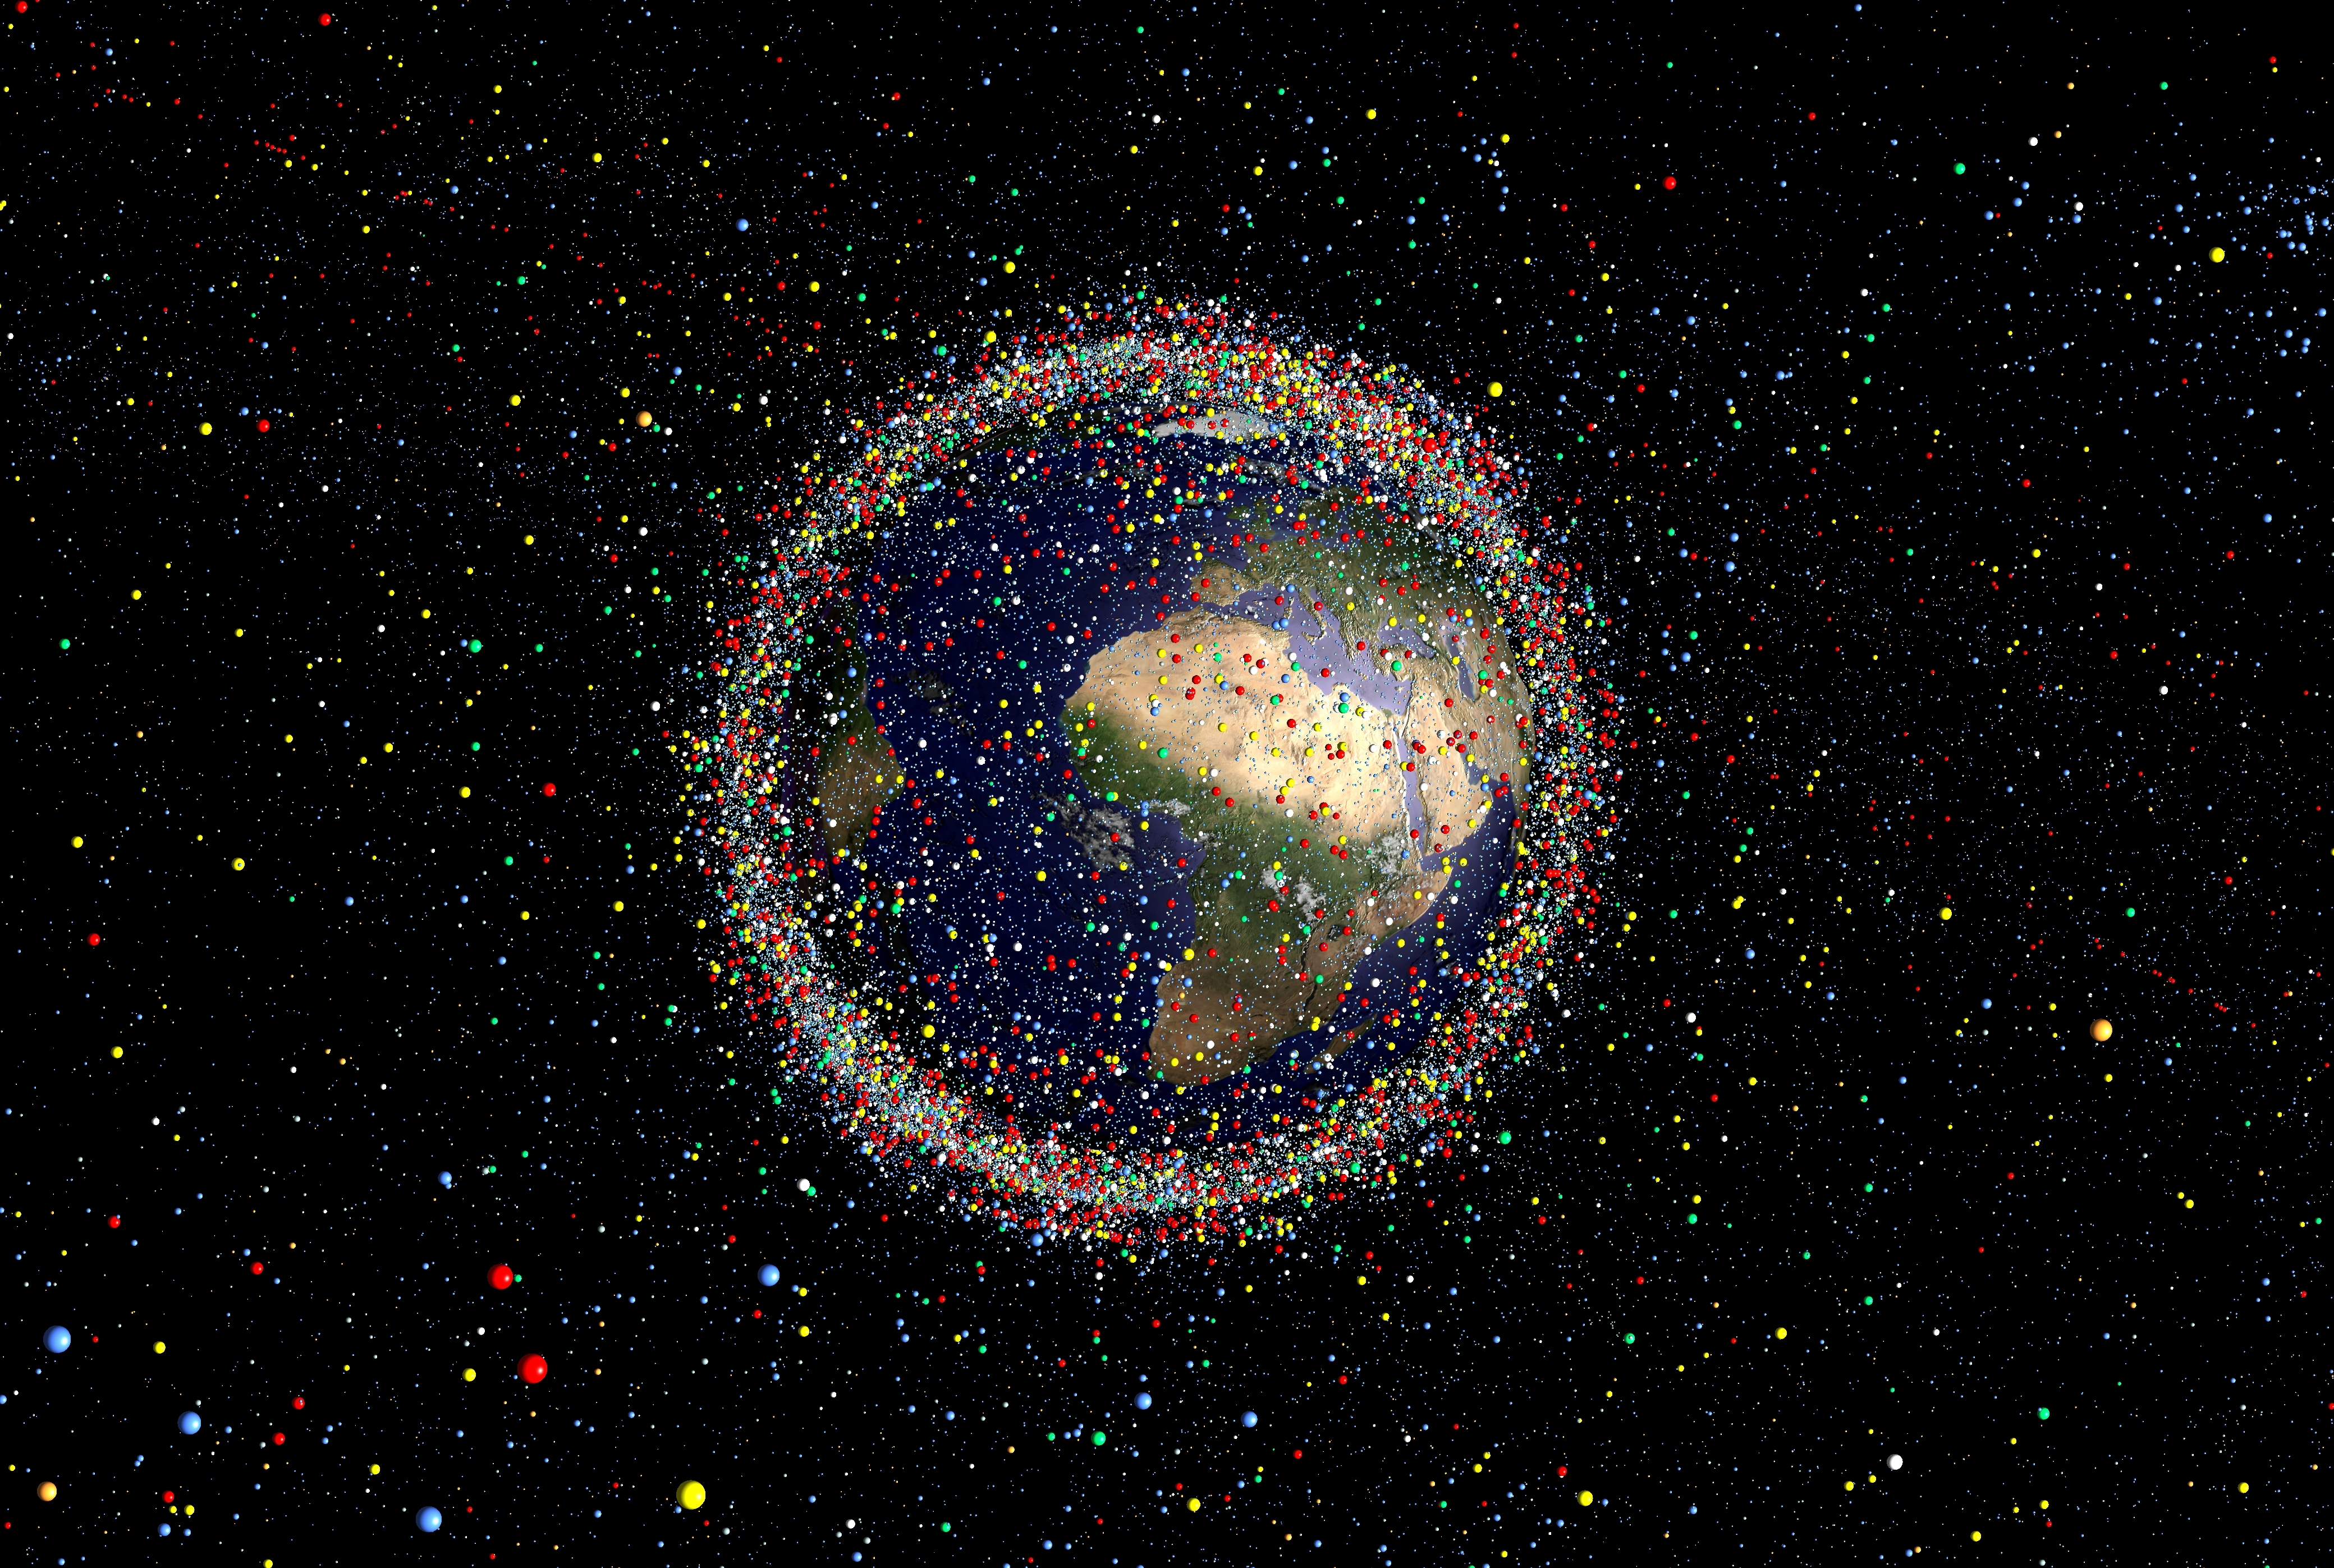
\includegraphics[scale=0.1]{./Sections_CD/S6-End_Of_Life/Images_S6/Picture_1_S6.jpg} 
\caption{View of the Space Debris around the Earth}
\end{figure}
\newline
\newline
 The category that concerns the project is the non-functional spacecraft because it refers to all intact structures which have completed their mission. It is noticed that once satellite’s operative lifetime arrives to its end, the satellites stop maneuvering and counteracting perturbations to maintain the current orbit. Consequently, they tend to deviate from their nominal orbital parameters, starting an unknown trajectory and important repercussions. 
\newline
\newline
Therefore, by increasing the number of uncontrolled \textit{``dead''} satellites the probability of collision between working satellites and space debris increases at LEO as it is overcrowded. Space debris is small usually and its location can be followed from earth but is impossible to control it. Meanwhile, it is essential for space assets to be free of any impact because avoidance maneuvers are too complicated to have real success.  Thereby, the increasing risk of collision becomes the big threat everyone is fighting against. 


\subsection{End-of-Life Types}

End-of-life strategies where implemented taking into account three factors: the time the satellite can orbit, the technical feasibility of active de-orbiting in terms of propellant and sub-systems enhancements and the altitude of its nominal orbital plane. 
\newline
\newline
The first one is related to the fact that the current recommendations say that any space asset that can become a non-functional spacecraft must de-orbit and disintegrate at its twenty-fifth birth on orbit. The second refers to the magnitude of the maneuver that can be developed with the power the thruster system can achieve. The third one is relevant because perturbations in space change according to the distance to the Earth’s surface. The closer it is the more perturbations from Earth and drag forces from the atmosphere the satellite suffers and perturbations help to de-orbit and disintegrate space assets.
\newline
\newline
Based on these premises, two different end-of-life groups had been determined: 

\begin{itemize}

\item[-] \textsc{Controlled de-orbit:}


It consists on performing a controlled re-entry by burning-up the satellite in the atmosphere or by driving the satellite to the ground in order to impact at a pre-assigned safe-location. 
This sophisticated maneuver is initiated by a large increment of potential energy to make change the orbital altitude to a lower one well into the atmosphere where the space debris will burn.

\item[-]  \textsc{Uncontrolled de-orbit:}

A simplest and cheaper way to de-orbit satellites is to induce a reduction of the orbit altitude to cause a decay and finally a re-entry. This maneuvre consists in de-orbiting the satellite by short maneuvres such as low-thrust maneuvres which help to decay the satellite position but without controlling its trajectory.
\newline
\newline
For satellites, which are placed at the LEO, this strategy takes advantage of LEO perturbations that assist in lowering the orbit altitude. This derivative of un-controlled de-orbit is known as the Non-propulsive orbit lifetime reduction. 
\newline

\emph{REMINDER:} the residual lifetime of the satellites has to be lower than 25 years.

\end{itemize} 

As \textsc{Astrea} constellation will be positioned at LEO those perturbations are useful to de-orbit the satellites due to the fact they actually burn-up in the atmosphere during the re-entry. 
\newline


\end{document} % Section 6: End Of Life